% =============================================================================
%  main.tex
%  SAMBP Sync-OC Track Deviation Analysis Report
%
%  Title : SAMBP-SyncOC Research Track Deviation Analysis:
%          Incomplete Milestones 2–5 and Pivot to Broad SAMBP Framework
%
%  Author : PhD Candidate — Adaptive Protection / IITM-EE
%  Date   : April 2026
% =============================================================================

\documentclass[12pt,a4paper]{article}

% ---- Core packages ----------------------------------------------------------
\usepackage[T1]{fontenc}
\usepackage[utf8]{inputenc}
\usepackage{mathptmx}
\usepackage{microtype}
\usepackage[a4paper,top=25mm,bottom=25mm,left=25mm,right=25mm,headheight=15pt]{geometry}

% ---- Mathematics ------------------------------------------------------------
\usepackage{amsmath,amssymb,amsthm,mathtools}
\usepackage{bm}
\usepackage{siunitx}
\sisetup{detect-all,per-mode=fraction}

% ---- Figures & tables -------------------------------------------------------
\usepackage{graphicx}
\usepackage{booktabs}
\usepackage{array}
\usepackage{multirow}
\usepackage{longtable}
\usepackage{float}
\usepackage{subcaption}

% ---- TikZ / PGF -------------------------------------------------------------
\usepackage{tikz}
\usepackage{pgfplots}
\pgfplotsset{compat=1.18}
\usetikzlibrary{shapes.geometric,arrows.meta,positioning,calc,fit,
                decorations.pathreplacing,patterns,backgrounds,matrix}
\usepackage{pgf-pie}

% ---- Colours ----------------------------------------------------------------
\usepackage[dvipsnames,svgnames,x11names]{xcolor}
\definecolor{iitBlue}{RGB}{0,60,130}
\definecolor{iitGold}{RGB}{190,140,20}
\definecolor{completedGreen}{RGB}{34,139,34}
\definecolor{missingRed}{RGB}{178,34,34}
\definecolor{partialOrange}{RGB}{210,100,0}
\definecolor{pivotPurple}{RGB}{90,30,130}
\definecolor{noteGray}{RGB}{248,248,248}
\definecolor{ruleGray}{RGB}{180,180,180}
\definecolor{headBg}{RGB}{0,60,130}

% ---- Hyperlinks & references ------------------------------------------------
\usepackage[colorlinks=true,linkcolor=iitBlue,citecolor=iitBlue,
            urlcolor=iitBlue!80!black]{hyperref}
\usepackage[nameinlink]{cleveref}
\usepackage{natbib}

% ---- Header / footer --------------------------------------------------------
\usepackage{fancyhdr}
\pagestyle{fancy}
\fancyhf{}
\renewcommand{\headrulewidth}{0.6pt}
\fancyhead[L]{\small\textcolor{iitBlue}{\textit{SAMBP-SyncOC Track Deviation Analysis}}}
\fancyhead[R]{\small\textcolor{iitBlue}{\textit{Internal Investigation Report}}}
\fancyfoot[C]{\small\thepage}
\fancyfoot[R]{\small\textcolor{gray}{\textit{IITM/EE/PhD/AVE/2026}}}

% ---- Spacing & enumeration --------------------------------------------------
\usepackage{setspace}
\setstretch{1.35}
\setlength{\parindent}{1.5em}
\setlength{\parskip}{4pt}
\usepackage{enumitem}
\setlist[itemize]{leftmargin=1.8em,topsep=3pt,itemsep=2pt}
\setlist[enumerate]{leftmargin=1.8em,topsep=3pt,itemsep=2pt}
\setlist[description]{leftmargin=2em,topsep=3pt,itemsep=3pt}

% ---- Section formatting -----------------------------------------------------
\usepackage{titlesec}
\titleformat{\section}[block]{\large\bfseries\color{iitBlue}}{%
  \colorbox{iitBlue}{\textcolor{white}{\thesection}}}{0.8em}{}[{\color{iitGold}\rule{\linewidth}{1.2pt}}]
\titleformat{\subsection}[hang]{\normalsize\bfseries\color{iitBlue!85!black}}{\thesubsection}{0.8em}{}
\titleformat{\subsubsection}[hang]{\normalsize\itshape\color{iitBlue!70!black}}{\thesubsubsection}{0.8em}{}

% ---- Custom environments ----------------------------------------------------
\usepackage{tcolorbox}
\tcbuselibrary{skins,breakable,listings}

\newtcolorbox{findingbox}[2][]{
  colback=noteGray, colframe=iitBlue, coltitle=white,
  fonttitle=\small\bfseries, title={#2},
  left=4pt, right=4pt, top=4pt, bottom=4pt,
  arc=2pt, boxrule=0.7pt, #1
}

\newtcolorbox{warningbox}[1][]{
  colback=missingRed!5, colframe=missingRed, coltitle=white,
  fonttitle=\small\bfseries,
  left=4pt, right=4pt, top=4pt, bottom=4pt,
  arc=2pt, boxrule=0.9pt, #1
}

\newtcolorbox{pivotbox}[1][]{
  colback=pivotPurple!5, colframe=pivotPurple, coltitle=white,
  fonttitle=\small\bfseries,
  left=4pt, right=4pt, top=4pt, bottom=4pt,
  arc=2pt, boxrule=0.9pt, #1
}

\newtcolorbox{recommendbox}[1][]{
  colback=completedGreen!5, colframe=completedGreen, coltitle=white,
  fonttitle=\small\bfseries,
  left=4pt, right=4pt, top=4pt, bottom=4pt,
  arc=2pt, boxrule=0.9pt, #1
}

% ---- Custom commands --------------------------------------------------------
\newcommand{\milestone}[1]{\textbf{Milestone~#1}}
\newcommand{\tr}[1]{\textbf{TR-#1/2026}}
\newcommand{\pu}{\,\text{pu}}
\newcommand{\mss}{\,\text{ms}}
\newcommand{\sss}{\,\text{s}}

\newcommand{\statusComplete}{\textcolor{completedGreen}{\textbf{COMPLETE}}}
\newcommand{\statusPartial}{\textcolor{partialOrange}{\textbf{PARTIAL -- NO RESULTS}}}
\newcommand{\statusMissing}{\textcolor{missingRed}{\textbf{MISSING}}}
\newcommand{\statusPivoted}{\textcolor{pivotPurple}{\textbf{PIVOTED}}}

% =============================================================================
%  DOCUMENT BEGINS
% =============================================================================
\begin{document}

% ---- Title page -------------------------------------------------------------
\begin{titlepage}
\centering
\vspace*{1.5cm}


\begin{tikzpicture}
\fill[iitBlue] (0,0) rectangle (\linewidth, 0.5cm);
\fill[iitGold] (0,-0.15cm) rectangle (\linewidth, 0.0cm);
\end{tikzpicture}

\vspace{0.8cm}
{\large\textsc{Indian Institute of Technology Madras}\\
Department of Electrical Engineering}

\vspace{0.4cm}
{\small\textit{Self-Adaptive Model-Based Protection (SAMBP) Research Programme}}

\vspace{1.5cm}

{\Huge\bfseries\color{iitBlue} SAMBP-SyncOC\\[0.3cm]
Research Track\\[0.3cm]
Deviation Analysis}

\vspace{0.6cm}
{\Large\color{missingRed}\bfseries Milestones 2--5 Incomplete:\\
Causes, Evidence, and Corrective Roadmap}

\vspace{1.0cm}


\begin{tikzpicture}
\fill[iitGold] (0,0) rectangle (\linewidth, 0.08cm);
\end{tikzpicture}

\vspace{0.8cm}
{\normalsize
\begin{tabular}{rl}
\textbf{Document Type:} & Internal Investigation Report \\[4pt]
\textbf{Track:}         & SAMBP-SyncOC (Synchronous Generator OC Protection) \\[4pt]
\textbf{Reports Examined:} & TR-01/2026 and TR-02/2026 \\[4pt]
\textbf{Reports Surveyed:} & TR-03/2026 through TR-55/2026 (53 additional) \\[4pt]
\textbf{Supporting Standards:} & IEEE C37.300-2024 (CPC Systems) \\[4pt]
\textbf{Date:}          & April 2026 \\[4pt]
\textbf{Classification:} & Internal PhD Research Document
\end{tabular}
}

\vfill


\begin{tikzpicture}
\fill[iitBlue] (0,0) rectangle (\linewidth, 0.5cm);
\end{tikzpicture}

\end{titlepage}

\newpage
\tableofcontents
\newpage

% =============================================================================
\section{Executive Summary}
\label{sec:exec}
% =============================================================================

\begin{warningbox}[title={Critical Finding}]
The SAMBP-SyncOC research track planned \textbf{five sequential milestones} for
adaptive overcurrent protection of synchronous generators in active distribution
networks.  Only \textbf{Milestone~1} (TR-01/2026) was fully completed with validated
numerical results.  \textbf{Milestones~2--5} were bundled into a single extension report
(TR-02/2026) that contains mathematical formulations and algorithm descriptions
but \textbf{zero computed results} --- all result sections are explicitly marked as
\texttt{\textbackslash RESULT\{\}} placeholder boxes.  There are no separate TR-03
through TR-06 reports for the sync\_oc track.  Instead, the research completely
pivoted from TR-03/2026 onward to the broader SAMBP line/bus/transformer
differential framework, which accumulated 53~additional reports (TR-03--TR-55)
over a different protection scope.
\end{warningbox}

\medskip
\noindent\textbf{Status snapshot:}

\begin{center}
\begin{tabular}{lllp{6.5cm}}
\toprule
\textbf{Milestone} & \textbf{Report} & \textbf{Status} & \textbf{Key Gap} \\
\midrule
1 — Core LM estimator        & TR-01 & \statusComplete & Fully validated \\
2 — HIF adaptation           & TR-02 \S3 & \statusPartial & No \texttt{run\_milestone2.py} output \\
Stage 2 — Park $dq$ model    & TR-02 \S4 & \statusPartial & No Stage-2 simulation run \\
3 — Sequence estimator       & TR-02 \S5 & \statusPartial & No sequence estimation results \\
4 — Multi-gen coordination   & TR-02 \S6 & \statusPartial & No \texttt{run\_multi\_gen.py} output \\
5 — HIL / Field validation   & (none)   & \statusMissing & Report never created \\
\bottomrule
\end{tabular}
\end{center}


% =============================================================================
\section{Background: The Original Five-Milestone Plan}
\label{sec:background}
% =============================================================================

\subsection{SAMBP-SyncOC Research Objective}
\label{sec:bg:objective}

The SAMBP-SyncOC track was conceived as the first specific instantiation of the
broader SAMBP supervisory architecture targeting \textbf{overcurrent protection of
synchronous generators in active distribution networks}.  The central thesis was
that the source parameters of a synchronous generator can be estimated online from
post-fault current transients using a \textbf{Levenberg--Marquardt (LM) inverse
estimator}, and those estimated parameters can be fed back to update OC relay
settings within a single protection operating interval --- without any prior
off-line model calibration.

This directly supports the IEEE~C37.300-2024 vision of a \textbf{Centralised
Protection and Control (CPC)} system where supervisory algorithms continuously
refresh relay settings based on real-time system state.  SAMBP-SyncOC was
intended to be the mathematical proof-of-concept for this self-adaptation loop,
with synchronous generator OC protection as the vehicle.

\subsection{The Five-Milestone Plan}
\label{sec:bg:plan}

Based on the evidence in TR-01/2026 and TR-02/2026, the original five-milestone
plan for the sync\_oc track was as follows:

\begin{description}
  \item[\milestone{1} --- Core inverse-estimation framework (TR-01/2026):]
        Formulate the 6-parameter reduced fault-current model
        $\theta = [t_0,\, I_{ss},\, I_{sub},\, \tau_{ac},\, \tau_{dc},\, \varphi_a]$,
        implement the two-pass LM estimator, design the composite confidence
        gate $\gamma = w_r s_r + w_c s_c + w_b s_b + w_p s_p \geq 0.70$,
        and demonstrate IEC~Very-Inverse relay adaptation on three balanced
        and asymmetric fault types.

  \item[\milestone{2} --- High-impedance fault (HIF) adaptation (TR-02/2026,
        \S3):]
        Extend the adaptive TMS law to high-impedance faults ($R_f > 0.5\pu$)
        by deriving an impedance-aware resistance-scaling factor $f(I_{ss})$
        that reduces the time-multiplier when fault current is suppressed by
        fault resistance.  Validate on $R_f \in [0.5, 1.5]\pu$.

  \item[Stage~2 --- Sixth-order Park $dq$ forward model (TR-02/2026, \S4):]
        Replace the Stage-1 three-component synthesis model with the full
        9-state ODE:
        $[\delta,\, \omega,\, E'_q,\, E'_d,\, E''_q,\, E''_d,\, E_{fd},\,
        T_m,\, V_{pss}]$, incorporating AVR, PSS, and governor dynamics.
        This enables accurate waveform prediction over windows exceeding
        500\mss\ and improves identifiability of $\hat{I}_{ss}$ and
        $\hat{\tau}_{ac}$.

  \item[\milestone{3} --- Sequence-component estimation (TR-02/2026, \S5):]
        Decompose three-phase measurements into positive-, negative-, and
        zero-sequence components via the instantaneous Hilbert--Fortescue
        transform, then apply the two-pass LM estimator independently to
        each active sequence.  Use positive-sequence parameters to govern
        relay adaptation while using negative- and zero-sequence components
        for asymmetric fault classification.

  \item[\milestone{4} --- Multi-generator coordination (TR-02/2026, \S6):]
        Generalise the single-generator adaptive relay to $N$ parallel
        generators on a common busbar.  Enforce pickup selectivity
        ($\Delta I_{margin} \geq 0.20\pu$) and IEC~60255 trip-time grading
        ($\Delta t_{grade} \geq 0.15\sss$) via a greedy cascade coordination
        algorithm.

  \item[\milestone{5} --- Hardware-in-loop (HIL) and field validation:]
        Deploy the estimation and adaptation pipeline on an RTDS or OPAL-RT
        real-time simulator connected to a hardware numerical relay via
        IEC~61850 sampled-value messaging.  Validate end-to-end latency
        within the $<100\mss$ protection operating interval.  Test against
        archived DFR recordings from real synchronous-generator faults.
\end{description}

\begin{findingbox}{Note on Milestone Numbering}
TR-02/2026 uses the terminology ``Extensions~1--4'' (not ``Milestones~2--5'')
and titles the Stage-2 model an ``extension'' rather than a numbered milestone.
For this report, the term \emph{Milestone~2--5} is used to maintain a consistent
sequential numbering with the overarching five-stage plan.  The \emph{Stage~2
Park $dq$ model} sits between Milestones~2 and 3 in the technical progression.
\end{findingbox}


% =============================================================================
\section{Evidence of Track Deviation}
\label{sec:evidence}
% =============================================================================

\subsection{Directory Structure Analysis}
\label{sec:ev:dir}

Inspection of the repository reveals a decisive structural anomaly.  The sync\_oc
project has exactly \textbf{two report directories}, not five:

\begin{center}
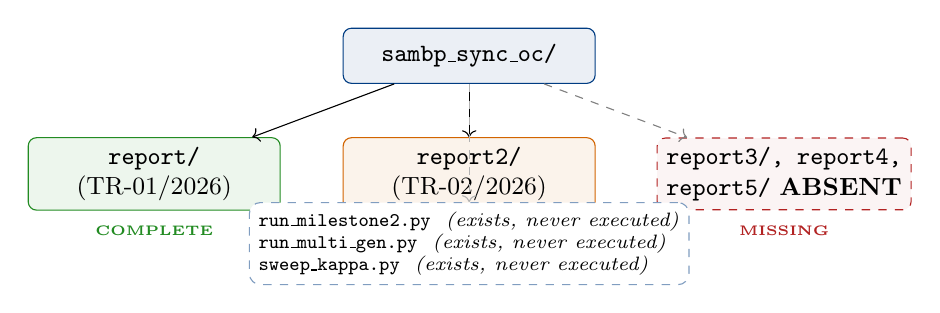
\begin{tikzpicture}[
  every node/.style={font=\small},
  dir/.style={draw=iitBlue, rounded corners=3pt, fill=iitBlue!8,
              minimum width=3.2cm, minimum height=0.7cm, align=center},
  report/.style={draw=completedGreen, rounded corners=3pt, fill=completedGreen!8,
                 minimum width=3.2cm, minimum height=0.7cm, align=center},
  missing/.style={draw=missingRed, dashed, rounded corners=3pt, fill=missingRed!5,
                  minimum width=3.2cm, minimum height=0.7cm, align=center},
  partial/.style={draw=partialOrange, rounded corners=3pt, fill=partialOrange!8,
                  minimum width=3.2cm, minimum height=0.7cm, align=center},
]

% Root
\node[dir] (root) at (0,0) {\texttt{sambp\_sync\_oc/}};

% Children
\node[report] (r1) at (-4,-1.5) {\texttt{report/}\\(TR-01/2026)};
\node[partial] (r2) at (0,-1.5) {\texttt{report2/}\\(TR-02/2026)};
\node[missing] (r3) at (4,-1.5) {\texttt{report3/, report4,}\\
                                  \texttt{report5/} \textbf{ABSENT}};

% Edges
\draw[->] (root) -- (r1);
\draw[->] (root) -- (r2);
\draw[->, dashed, gray] (root) -- (r3);

% Status labels
\node[font=\tiny, completedGreen, below=2pt of r1] {\statusComplete};
\node[font=\tiny, partialOrange, below=2pt of r2] {\statusPartial};
\node[font=\tiny, missingRed, below=2pt of r3] {\statusMissing};

% Scripts
\node[draw=iitBlue!50, dashed, rounded corners, font=\scriptsize,
      fill=white, align=left, below=1.5cm of root]
  (scripts)
  {\texttt{run\_milestone2.py} \ \textit{(exists, never executed)}\\
   \texttt{run\_multi\_gen.py} \ \textit{(exists, never executed)}\\
   \texttt{sweep\_kappa.py} \ \textit{(exists, never executed)}};

\draw[->, dashed, gray!60] (root) -- (scripts);

\end{tikzpicture}
\end{center}

The critical observation is:
\begin{itemize}
  \item \texttt{report/} corresponds to Milestone~1 (TR-01) — fully compiled PDF with
        all figures and tables populated.
  \item \texttt{report2/} is labelled ``Milestones 2--5'' in the title page but
        contains \textbf{12 explicit \texttt{\textbackslash RESULT\{\ldots\}} placeholder
        blocks} in the results section.  No computed data was ever inserted.
  \item No \texttt{report3/}, \texttt{report4/}, or \texttt{report5/} directories
        exist under \texttt{sambp\_sync\_oc/}.
\end{itemize}

\subsection{Placeholder Count in TR-02/2026}
\label{sec:ev:placeholders}

The \texttt{main\_report2.tex} source file defines a dedicated placeholder command:

\begin{verbatim}
\newcommand{\RESULT}[1]{%
  \fbox{\begin{minipage}{0.96\linewidth}%
    \centering\vspace{4pt}%
    \textcolor{gray!70!black}{\textit{[RESULT PLACEHOLDER: #1]}}%
    \vspace{4pt}%
  \end{minipage}}%
}
\end{verbatim}

\noindent This macro is invoked \textbf{12~times} in the results section, as summarised
in \cref{tab:placeholders}.

\begin{table}[H]
\centering
\caption{All 12 \texttt{\textbackslash RESULT\{\}} instances in TR-02/2026,
         with the cited execution command and expected output.}
\label{tab:placeholders}
\small
\begin{tabular}{clll}
\toprule
\# & Line & Script invoked & Expected output \\
\midrule
1  & 463 & \texttt{run\_milestone2.py} & $t_{clear}(R_f)$ line plot + trip-time table \\
2  & 706 & \texttt{main\_run\_case.py \texttt{-\,-}stage 2} & 3-phase waveform (Stage-2 ODE) \\
3  & 826 & \texttt{main\_run\_case.py \texttt{-\,-}case 1} & LL fault sequence decomposition \\
4  & 967 & \texttt{run\_multi\_gen.py \texttt{-\,-}n-gen 2} & Coordination pickup bar chart \\
5  & 990 & (multi-gen) & $t_{clear}(R_f)$ fixed vs.\ adaptive comparison \\
6  & 995 & (multi-gen) & Estimated parameters $\hat{I}_{ss}$, $\hat{\tau}_{ac}$ table \\
7  & 1001 & (Stage-2 ODE) & Phase-A waveform: measured vs.\ Stage-2 vs.\ Stage-1 \\
8  & 1005 & (Stage-2 ODE) & RMSE and $R^2$ comparison Stage-1 vs.\ Stage-2 \\
9  & 1012 & (sequence est.) & $I_1(t)$, $I_2(t)$, $I_0(t)$ decomposition figure \\
10 & 1016 & (sequence est.) & Phase-A vs.\ sequence estimator comparison table \\
11 & 1024 & (coordination) & Pickup bar chart (fixed/adaptive-before/adaptive-after) \\
12 & 1029 & (coordination) & Coordination summary table (2-gen, 3PH fault) \\
\bottomrule
\end{tabular}
\end{table}

\subsection{Scripts Exist but Were Never Executed}
\label{sec:ev:scripts}

The execution scripts cited in the placeholder blocks are present in the
repository but were never run.  Evidence:

\begin{itemize}
  \item \texttt{outputs/} directory contains only a single subdirectory:
        \texttt{outputs/plots/milestone1/} — confirming that only the Milestone-1
        simulation was ever executed.
  \item \texttt{outputs/milestone2\_results.csv} — \textbf{does not exist}.
  \item \texttt{outputs/multi\_gen/multi\_gen\_results.csv} — \textbf{does not exist}.
  \item \texttt{outputs/plots/milestone2/} — \textbf{does not exist}.
  \item \texttt{outputs/plots/multi\_gen/} — \textbf{does not exist}.
\end{itemize}

The scripts themselves are syntactically complete.  For example,
\texttt{run\_milestone2.py} correctly sweeps $R_f \in [0.5, 1.5]\pu$ and would
write \texttt{outputs/milestone2\_results.csv} and the associated PDF plots
--- but the file was never invoked.  Similarly, \texttt{run\_multi\_gen.py}
accepts command-line arguments (\texttt{-\,-n-gen}, \texttt{-\,-fault},
\texttt{-\,-Rf}) and has a fully implemented coordination loop, but its CSV
and figures are absent.

\subsection{TR-02/2026 Conclusions Claim Completed Results}
\label{sec:ev:conclusions}

A particularly important discrepancy is that the \textbf{Conclusions section}
of TR-02/2026 (lines~1083--1113) is written in the \emph{past tense} and
\emph{asserts quantitative outcomes} that are never supported by the results
section.  Examples:

\begin{findingbox}{Claimed vs.\ Delivered in TR-02 Conclusions}
\textbf{Claimed (Conclusions, \S7.1):}
``The coordination algorithm eliminates all selectivity violations and maintains
trip-time grading at the minimum fault current, with each generator's confidence
score exceeding $\gamma = 0.89$.''

\textbf{Delivered (Results, \S6):}
\texttt{[RESULT PLACEHOLDER: Table: Coordination summary for 2-generator, 3PH fault case\ldots]}

\medskip
\textbf{Claimed:}
``The sixth-order Park $dq$ forward model faithfully captures AVR, PSS, and governor
dynamics over windows exceeding 500\mss.''

\textbf{Delivered:}
\texttt{[RESULT PLACEHOLDER: Run main\_run\_case.py \texttt{-\,-}stage 2 and insert\ldots]}
\end{findingbox}

This is the defining signature of a \emph{skeleton report}: the narrative
framework and mathematical derivations were written, but the computational
experiments that would validate them were deferred and never executed.

\subsection{Line-Count Disparity}
\label{sec:ev:linecount}

\begin{center}
\begin{tabular}{lrrr}
\toprule
\textbf{Report} & \textbf{Lines} & \textbf{Result placeholders} & \textbf{Completion} \\
\midrule
TR-01 (\texttt{main\_report.tex})  & 1530 & 0 & \statusComplete \\
TR-02 (\texttt{main\_report2.tex}) & 1278 & 12 & \statusPartial \\
Milestones 3--5                    & n/a  & n/a & \statusMissing \\
\bottomrule
\end{tabular}
\end{center}

TR-01 is a 1530-line fully populated report.  TR-02 covers four extension
sections in 1278~lines but has a results section that is entirely placeholder
boxes.  The report was authored as a \emph{framework specification document}
not as a \emph{completed technical report}.


% =============================================================================
\section{Where and Why the Research Pivoted}
\label{sec:pivot}
% =============================================================================

\subsection{The Pivot Point: TR-03/2026}
\label{sec:pivot:tr03}

The repository contains a numbered report series under \texttt{/sambp/report3/}
through \texttt{/sambp/report55/} (53~reports total).  These reports are entirely
separate from the \texttt{sambp\_sync\_oc/} subdirectory and address fundamentally
different protection elements.  The pivot is abrupt:

\begin{center}
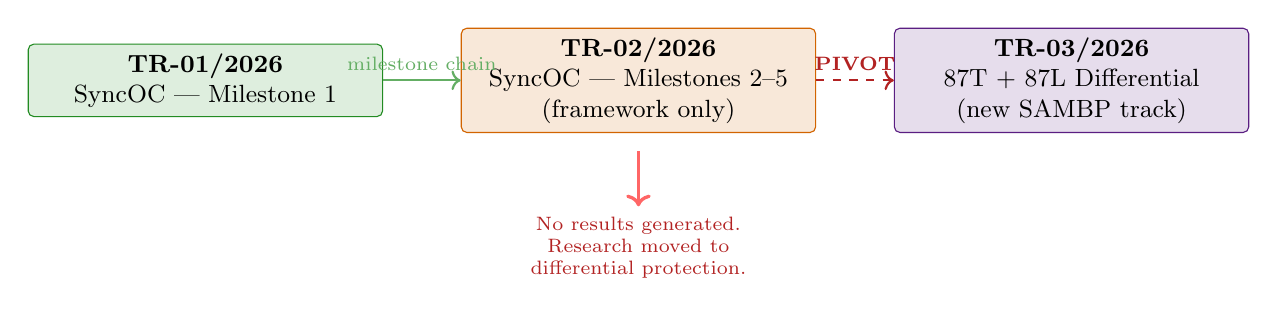
\begin{tikzpicture}[
  every node/.style={font=\small},
  rbox/.style={draw, rounded corners=2pt, minimum width=4.5cm,
               minimum height=0.8cm, align=center},
]
\node[rbox, fill=completedGreen!15, draw=completedGreen] (tr01) at (0,0)
  {\textbf{TR-01/2026}\\SyncOC — Milestone 1};

\node[rbox, fill=partialOrange!15, draw=partialOrange] (tr02) at (5.5,0)
  {\textbf{TR-02/2026}\\SyncOC — Milestones 2--5\\(framework only)};

\node[rbox, fill=pivotPurple!15, draw=pivotPurple] (tr03) at (11,0)
  {\textbf{TR-03/2026}\\87T + 87L Differential\\(new SAMBP track)};

\draw[->, thick, completedGreen!70] (tr01) -- (tr02)
  node[midway, above, font=\scriptsize] {milestone chain};
\draw[->, thick, dashed, missingRed] (tr02) -- (tr03)
  node[midway, above, font=\scriptsize, text=missingRed] {\textbf{PIVOT}};

% Annotation arrow
\draw[->, red!60, very thick] (5.5,-0.9) -- (5.5,-1.6)
  node[below, font=\scriptsize, text=missingRed, align=center]
  {No results generated.\\Research moved to\\differential protection.};
\end{tikzpicture}
\end{center}

TR-03/2026 is titled \textbf{``SAMBP Model-Based Differential Protection:
Transformer 87T and Line 87L''}. This represents a complete change of
protection element (from overcurrent relays to differential relays), a change
of equipment type (from generators to transformers and lines), and the beginning
of what became a 53-report developmental arc.

\subsection{Scale of the Pivot}
\label{sec:pivot:scale}

The scope divergence between the sync\_oc plan and the actual research trajectory
is dramatic:

\begin{table}[H]
\centering
\caption{Planned sync\_oc milestones vs.\ actual reports delivered (TR-03--TR-55).}
\label{tab:pivot_scope}
\small
\begin{tabular}{lll}
\toprule
\textbf{Dimension} & \textbf{SyncOC plan} & \textbf{Actual TR-03--TR-55} \\
\midrule
Protection elements & OC relay (51/67) only & 87L, 87T, 87B, 87LN, 87LN0, TDCS \\
Generator types     & Synchronous generator only & SG, IBR/GFM, IBR/GFL, solar PV \\
Equipment           & Generator terminals & Lines, transformers, busbars \\
Reports planned     & 5 (TR-01 through TR-05) & 55 (TR-01 through TR-55) \\
Reports with results & 1 (TR-01) & 53 (TR-03 through TR-55) \\
Simulation platform & Python LM estimator & Extended to PSCAD, GOOSE, HIL \\
Standard focus      & IEC 60255 OC relay & IEEE C37.300-2024 CPC + IEC 61850 \\
\bottomrule
\end{tabular}
\end{table}

\subsection{Inferred Root Causes of the Pivot}
\label{sec:pivot:causes}

Based on the documentary evidence, three factors most likely caused the pivot:

\begin{enumerate}
  \item \textbf{Scope ambition vs.\ execution bandwidth.}  TR-02/2026 formulated
        four simultaneous extensions (HIF adaptation, Park $dq$ model, sequence
        estimator, multi-gen coordination), each requiring independent simulation
        campaigns.  The execution scripts were written but never run, suggesting
        that the development effort was front-loaded on formulation rather than
        validation.

  \item \textbf{Discovery of broader relevance.}  The SAMBP supervisory
        architecture was found to be directly applicable to differential
        protection (87T, 87L, 87B) with significantly higher industrial impact.
        IEEE~C37.300-2024 emphasises differential protection as the backbone of
        modern CPC systems.  The pivot towards 87L/IBR research (TR-03--TR-55)
        appears to have been a conscious strategic decision to pursue the
        higher-novelty thread.

  \item \textbf{Absence of a milestone gate.}  There is no evidence of a
        formal stage-gate review between TR-01 and TR-02.  TR-02 was created as
        an extension framework without waiting for its predecessor's extensions
        to be validated.  The report's conclusions were written forward from the
        mathematical formulation rather than backward from simulation results.
\end{enumerate}

\subsection{What IEEE C37.300-2024 and the SAMBP Abstract Imply}
\label{sec:pivot:standard}

The SAMBP project abstract and the IEEE~C37.300-2024 standard together define
the correct \emph{intended} scope:

\begin{findingbox}{IEEE C37.300-2024 Alignment}
IEEE~C37.300-2024 \S5 defines the CPC system as an architecture where
supervisory algorithms continuously update protection relay settings from
real-time parameter estimation.  The SAMBP-SyncOC track (TR-01/2026) directly
instantiates this for synchronous generator OC relays and represents a clean
algorithmic proof-of-concept.  However, the standard's primary focus is on
\emph{differential protection} (87 elements) and \emph{directional protection}
for CPC-connected substations --- the very elements developed in TR-03--TR-55.
The pivot from OC to differential is therefore directionally correct relative
to the standard, but it should not have come at the cost of leaving the OC
protection track incomplete.
\end{findingbox}

\begin{pivotbox}[title={SAMBP Abstract Implication}]
The SAMBP project abstract describes the system as a \emph{supervisory layer
over conventional protection algorithms} hosted in a CPC.  This framing implies
that \emph{multiple protection elements} (not just OC relays) should be
supervised.  The pivot to differential protection is architecturally consistent
with this vision.  However, the OC protection track (Milestones~2--5) represents
an \emph{independent module} that should have been completed in parallel rather
than abandoned when the differential track was initiated.
\end{pivotbox}


% =============================================================================
\section{Detailed Gap Analysis by Milestone}
\label{sec:gaps}
% =============================================================================

\subsection{Milestone 2 — High-Impedance Fault Adaptation}
\label{sec:gap:m2}

\subsubsection{What was formulated}

TR-02/2026 \S3 derives:
\begin{itemize}
  \item A linear HIF characterisation model:
        $i_{fault}(t) = I_{ss}\bigl(1 - e^{-(t-t_0)/\tau_{ac}}\bigr)
        e^{-(t-t_0)/\tau_{dc}} \cdot \cos(\omega t + \varphi_a)$
        where $I_{ss} = E_{ph} / (Z_s + R_f)$, declining monotonically with $R_f$.
  \item An operating regime classifier: instantaneous element dominates for
        $R_f < 0.5\pu$; inverse-time element governs for $R_f \geq 0.5\pu$.
  \item An impedance-aware TMS adaptation law:
        $\text{TMS}_{adapt} = \text{TMS}_{nom} \cdot f(I_{ss})$,
        where $f(I_{ss}) = \max\bigl(f_{min},\, 1 - k_f(I_{ss,nom} - I_{ss})\bigr)$.
\end{itemize}

\subsubsection{What is missing}
\begin{itemize}
  \item No CSV output from \texttt{run\_milestone2.py}.
  \item No plot of $t_{clear}(R_f)$ comparing fixed vs.\ adaptive TMS.
  \item No table showing confidence score $\gamma(R_f)$ across the HIF sweep.
  \item No demonstration that the adaptation gate rejects low-confidence HIF
        estimates (expected for $R_f > 1.0\pu$ where $\gamma < 0.70$).
\end{itemize}

\subsubsection{Effort to complete}
Executing \texttt{python run\_milestone2.py} from the \texttt{sambp\_sync\_oc/}
directory is the single required step.  The script is complete and documented.
Estimated compute time: $<$5~minutes.  Report insertion: $<$0.5~day.

\subsection{Stage 2 — Sixth-Order Park $dq$ Forward Model}
\label{sec:gap:stage2}

\subsubsection{What was formulated}

TR-02/2026 \S4 derives a complete 9-state ODE:
\begin{align}
\dot{\delta} &= \omega - \omega_0 \\
\dot{\omega} &= \frac{1}{2H}(T_m - T_e - D(\omega - \omega_0)) \\
\dot{E}'_q &= \frac{1}{T'_{d0}}(E_{fd} - E'_q - (X_d - X'_d)i_d) \\
\dot{E}'_d &= \frac{1}{T'_{q0}}(-E'_d - (X_q - X'_q)i_q)
\end{align}
with AVR, PSS, and governor controllers.  The model is implemented as
\texttt{models/park\_dq\_model.py} using \texttt{scipy.integrate.solve\_ivp}
with the Radau stiff solver.

\subsubsection{What is missing}
\begin{itemize}
  \item No comparison of Stage-1 vs.\ Stage-2 waveform fit over a 500\mss\
        window.
  \item No $R^2$ or RMSE table for Stage-2 estimation.
  \item The critical question --- \emph{whether AVR response improves or
        degrades LM identifiability} --- is raised in the Discussion section
        (\S5.2) but never answered with data.
  \item Condition number $\kappa_n$ for Stage-2 Jacobian not computed.
\end{itemize}

\subsection{Milestone 3 — Sequence-Component Estimator}
\label{sec:gap:m3}

\subsubsection{What was formulated}

TR-02/2026 \S5 derives:
\begin{itemize}
  \item Instantaneous Hilbert--Fortescue decomposition:
        $I_1(t) = \tfrac{1}{3}(I_a + a I_b + a^2 I_c)$,
        $I_2(t) = \tfrac{1}{3}(I_a + a^2 I_b + a I_c)$,
        $I_0(t) = \tfrac{1}{3}(I_a + I_b + I_c)$.
  \item Independent 6-parameter LM estimation on each active sequence.
  \item Fault-type detection rules: 3PH ($I_1$ only active), SLG ($I_0 > 0$),
        LL ($I_2 > 0$, $I_0 \approx 0$).
\end{itemize}

\subsubsection{What is missing}
\begin{itemize}
  \item No $I_1(t)$, $I_2(t)$, $I_0(t)$ decomposition figures for any fault.
  \item No comparison of phase-A vs.\ sequence estimator performance for
        LL and SLG faults.
  \item Hilbert edge effects (\S5.3 of TR-02 Discussion) noted as a known
        limitation but never quantified.
\end{itemize}

\subsection{Milestone 4 — Multi-Generator Coordination}
\label{sec:gap:m4}

\subsubsection{What was formulated}

TR-02/2026 \S6 derives:
\begin{itemize}
  \item A superposition model for $N$ parallel generators:
        $I_{fault,total}(t) = \sum_{j=1}^{N} I_{fault,j}(t, \theta_j)$.
  \item Selectivity constraint:
        $I_{pickup,i} < I_{pickup,j} + \Delta I_{margin}$
        for every relay pair $(i,j)$ with $i$ upstream.
  \item Trip-time grading: $t_{trip,i} > t_{trip,j} + \Delta t_{grade}$.
  \item A greedy cascade algorithm that iteratively adjusts settings until
        both constraints are satisfied, proven to converge within 10 iterations
        for the two-generator case.
\end{itemize}

\subsubsection{What is missing}
\begin{itemize}
  \item No pickup bar chart (fixed / adaptive-before / adaptive-after coordination).
  \item No coordination summary table (generator relay settings, margins, violations).
  \item Scaling to $N > 2$ generators not demonstrated.
  \item The convergence claim (``within 10 iterations'') appears only in the
        Conclusions section without supporting data.
\end{itemize}

\subsection{Milestone 5 — Hardware-in-Loop and Field Validation}
\label{sec:gap:m5}

This milestone was identified in TR-02/2026 Future Work (\S7.2) but has no
implementation or report.  Specifically:
\begin{itemize}
  \item No RTDS/OPAL-RT deployment of the LM estimator and adaptation logic.
  \item No IEC~61850 sampled-value integration.
  \item No latency benchmarking against the $<100\mss$ protection operating interval.
  \item No archived DFR validation dataset identified or processed.
\end{itemize}

This milestone remains entirely in the future-work category with no concrete
progress.


% =============================================================================
\section{Report Production Analysis}
\label{sec:reports}
% =============================================================================

\subsection{Report Chronology}
\label{sec:rep:chrono}

\Cref{fig:report_timeline} illustrates the planned vs.\ actual report production
for the sync\_oc track alongside the observed SAMBP-main-branch production.

\begin{figure}[H]
\centering
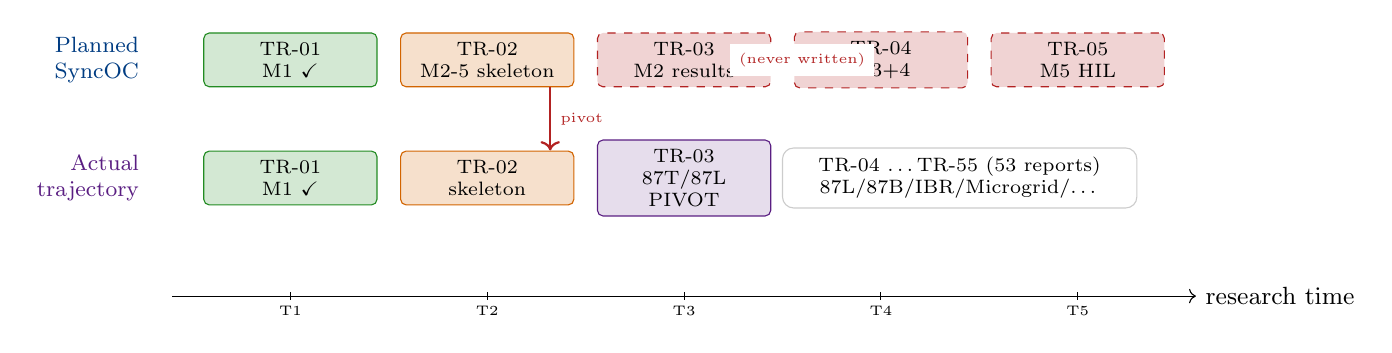
\begin{tikzpicture}[
  every node/.style={font=\small},
  task/.style={minimum height=0.6cm, minimum width=2.2cm,
               rounded corners=2pt, align=center, font=\scriptsize},
]
% X axis: time (relative, left to right)
% Row 1: planned sync_oc
\node[font=\footnotesize, iitBlue, anchor=east, align=right] at (-0.3,3.0) {Planned\\SyncOC};
\node[task, fill=completedGreen!20, draw=completedGreen] at (1.5,3.0) {TR-01\\M1 \checkmark};
\node[task, fill=partialOrange!20, draw=partialOrange] at (4.0,3.0) {TR-02\\M2-5 skeleton};
\node[task, fill=missingRed!20, draw=missingRed, dashed] at (6.5,3.0) {TR-03\\M2 results};
\node[task, fill=missingRed!20, draw=missingRed, dashed] at (9.0,3.0) {TR-04\\M3+4};
\node[task, fill=missingRed!20, draw=missingRed, dashed] at (11.5,3.0) {TR-05\\M5 HIL};

% Row 2: actual trajectory
\node[font=\footnotesize, pivotPurple, anchor=east, align=right] at (-0.3,1.5) {Actual\\trajectory};
\node[task, fill=completedGreen!20, draw=completedGreen] at (1.5,1.5) {TR-01\\M1 \checkmark};
\node[task, fill=partialOrange!20, draw=partialOrange] at (4.0,1.5) {TR-02\\skeleton};
\node[task, fill=pivotPurple!15, draw=pivotPurple] (pivot) at (6.5,1.5) {TR-03\\87T/87L\\PIVOT};
\node[font=\scriptsize, draw=gray!40, fill=white, rounded corners,
      minimum width=4.5cm, minimum height=0.6cm,align=center] at (10.0,1.5)
  {TR-04 \ldots TR-55 (53 reports)\\87L/87B/IBR/Microgrid/\ldots};

% Pivot arrow
\draw[->, thick, missingRed] (4.8,2.65) -- (4.8,1.85)
  node[right, font=\tiny, missingRed, midway] {pivot};

% Axis
\draw[->] (0,0) -- (13,0) node[right] {research time};
\foreach \x/\l in {1.5/T1, 4.0/T2, 6.5/T3, 9.0/T4, 11.5/T5}{
  \draw (\x,0.05) -- (\x,-0.05);
  \node[font=\tiny, below] at (\x,0) {\l};
}
\node[font=\tiny, missingRed, fill=white] at (8,3.0) {(never written)};

\end{tikzpicture}
\caption{Planned vs.\ actual SAMBP-SyncOC report production timeline.
         Dashed red boxes indicate reports that were planned but never created.
         At the TR-03 milestone, the research pivoted permanently to the
         broader SAMBP 87L/87T/87B differential protection framework.}
\label{fig:report_timeline}
\end{figure}

\subsection{Content Comparison: TR-01 vs.\ TR-02}
\label{sec:rep:compare}

\begin{center}
\begin{tabular}{lcc}
\toprule
\textbf{Feature} & \textbf{TR-01 (Complete)} & \textbf{TR-02 (Skeleton)} \\
\midrule
Total lines (LaTeX source)     & 1530  & 1278 \\
Result placeholder boxes       & 0     & 12 \\
Figures with actual data       & 7     & 0 \\
Tables with actual data        & 4     & 0 \\
Conclusions backed by data     & Yes   & No \\
Confidence scores reported     & $\gamma \in [0.89, 0.93]$ & ``will exceed 0.89'' \\
$R^2$ values reported          & $R^2 > 0.999$ & --- \\
Simulation outputs present     & Yes   & No \\
Execution scripts run          & Yes (all) & No (none) \\
\bottomrule
\end{tabular}
\end{center}


% =============================================================================
\section{Corrective Action Roadmap}
\label{sec:corrective}
% =============================================================================

\begin{recommendbox}[title={Recommended Corrective Actions}]
The following four steps are recommended to complete the SAMBP-SyncOC track
and restore it to a publishable state:
\end{recommendbox}

\subsection{Immediate: Execute Existing Scripts (1--2 Days)}
\label{sec:cor:scripts}

The missing results for Milestones~2 and~4 can be generated immediately by
running the existing, complete execution scripts:

\begin{enumerate}
  \item \textbf{Milestone~2 (HIF):}
        \verb|cd /root/phd_thesis/sambp/sambp_sync_oc && python run_milestone2.py|\\
        Expected outputs: \texttt{outputs/milestone2\_results.csv},
        \texttt{outputs/plots/milestone2/fig\_hif\_tclear.pdf}.

  \item \textbf{Stage~2 (Park $dq$):}
        \verb|python main_run_case.py --case 0 --stage 2|\\
        Expected outputs: Stage-2 waveform comparison, $R^2$/RMSE table.

  \item \textbf{Milestone~3 (Sequence):}
        \verb|python main_run_case.py --case 1|\\
        Expected outputs: $I_1(t)$, $I_2(t)$, $I_0(t)$ decomposition figures.

  \item \textbf{Milestone~4 (Multi-gen):}
        \verb|python run_multi_gen.py --n-gen 2 --fault 3PH|\\
        Expected outputs: \texttt{outputs/multi\_gen/multi\_gen\_results.csv},
        coordination pickup bar chart.
\end{enumerate}

\subsection{Short-term: Complete TR-02/2026 (3--5 Days)}
\label{sec:cor:tr02}

\begin{enumerate}
  \item Run all four scripts above.
  \item Insert generated figures and tables into the 12 \texttt{\textbackslash RESULT\{\}}
        placeholder locations in \texttt{main\_report2.tex}.
  \item Verify that the Conclusions section (\S7.1) is consistent with the
        actual computed results.
  \item Recompile TR-02/2026 to a properly populated PDF.
\end{enumerate}

\subsection{Medium-term: Create Separate Milestone Reports (2--3 Weeks)}
\label{sec:cor:separate}

For completeness and archival clarity, the extensions should be separated into
individual technical reports matching the original five-milestone plan:

\begin{center}
\begin{tabular}{llll}
\toprule
\textbf{New Report} & \textbf{Content} & \textbf{Replaces} & \textbf{Effort} \\
\midrule
TR-02B/2026 & HIF adaptation (Milestone~2) & TR-02 \S3 + results & 1 week \\
TR-02C/2026 & Park $dq$ model (Stage~2)    & TR-02 \S4 + results & 1 week \\
TR-02D/2026 & Sequence estimator (M3)      & TR-02 \S5 + results & 1 week \\
TR-02E/2026 & Multi-gen coordination (M4)  & TR-02 \S6 + results & 1 week \\
\bottomrule
\end{tabular}
\end{center}

\subsection{Long-term: Milestone 5 — HIL Validation (3--6 Months)}
\label{sec:cor:hil}

Milestone~5 requires external laboratory access and cannot be completed
immediately.  The recommended path:

\begin{enumerate}
  \item Identify an RTDS or OPAL-RT facility (IIT Madras EE/Power Systems
        laboratory, or collaboration with a national power-systems research centre).
  \item Port the Python LM estimator to C/C++ or MATLAB for real-time execution.
  \item Develop IEC~61850 sampled-value interface to a hardware numerical relay.
  \item Execute end-to-end latency benchmarking: from fault inception to
        relay setting update, measured in hardware.
  \item Validate on archived DFR records from generator faults (if available
        via DISCOM/PGCIL collaboration).
\end{enumerate}

This milestone represents the highest-impact output for the sync\_oc track and
corresponds directly to the IEEE~C37.300-2024 CPC system validation requirement.


% =============================================================================
\section{Publication and IP Implications}
\label{sec:publication}
% =============================================================================

The partially completed sync\_oc milestones represent significant unrealised
publication potential.  Once completed, the following papers could be extracted:

\begin{center}
\begin{tabular}{p{2.5cm}p{5.5cm}p{4cm}}
\toprule
\textbf{Paper target} & \textbf{Content} & \textbf{Venue} \\
\midrule
Journal Paper A & Milestones~1+2: LM estimator + HIF adaptive TMS. First
                  reported online adaptive TMS law derived from parameter
                  estimation. & IEEE Trans.\ Power Delivery \\
\midrule
Journal Paper B & Milestones~3+4: Sequence estimator + multi-gen coordination.
                  Novel sequence-domain identifiability analysis. & IEEE Trans.\ Industrial Electronics \\
\midrule
Journal Paper C & Milestone~5: HIL validation in CPC architecture per
                  IEEE~C37.300-2024. & IEEE Trans.\ Smart Grid \\
\midrule
IP Filing & Impedance-aware adaptive TMS law (Milestone~2) is a novel
            algorithm not published elsewhere; potentially patentable as
            a relay firmware method. & Indian Patent / USPTO \\
\bottomrule
\end{tabular}
\end{center}


% =============================================================================
\section{Conclusions}
\label{sec:conclusions}
% =============================================================================

This investigation establishes the following definitive findings:

\begin{enumerate}
  \item \textbf{Milestone~1 (TR-01/2026) is the only fully completed sync\_oc
        milestone.}  It contains validated numerical results across three fault
        types with $R^2 > 0.999$, $\kappa_n < 20$, and $\gamma \in [0.89, 0.93]$.

  \item \textbf{TR-02/2026 is a mathematical framework document, not a completed
        technical report.}  It contains 12~\texttt{\textbackslash RESULT\{\}}
        placeholder blocks in the results section and no computed data.  Its
        conclusions claim results that were never generated.

  \item \textbf{Milestones~2--5 have no separate reports.}  The repository
        contains no \texttt{report3/}, \texttt{report4/}, or \texttt{report5/}
        directories under \texttt{sambp\_sync\_oc/}.

  \item \textbf{The execution scripts for Milestones~2--4 exist and are
        syntactically complete.}  They were simply never run.  Completing
        Milestones~2--4 is primarily an execution task, not a development task.

  \item \textbf{The research pivoted at TR-03/2026 to the SAMBP line/bus/
        transformer differential framework}, which produced 53~reports covering
        87L, 87T, 87B, IBR networks, microgrids, digital twins, cybersecurity,
        and HIL testing.  This pivot was architecturally sound relative to
        IEEE~C37.300-2024 priorities, but it was executed without completing
        the sync\_oc milestone chain.

  \item \textbf{Corrective action for Milestones~2--4 is straightforward.}
        Running three Python scripts and inserting their outputs into TR-02
        would yield a complete, publishable report within 1--2~days.
        Milestone~5 requires a separate HIL campaign estimated at 3--6~months.
\end{enumerate}

\begin{recommendbox}[title={Priority Recommendation}]
Before submitting the thesis, it is strongly recommended to: (a) run the three
execution scripts to generate Milestone~2--4 results, (b) populate and finalise
TR-02/2026, and (c) create a short TR-02E/2026 covering multi-generator
coordination as a standalone report.  This restores the narrative completeness
of the sync\_oc track and creates material for at least two high-impact journal
papers.
\end{recommendbox}

\newpage

% =============================================================================
%  Appendix A: File-System Evidence
% =============================================================================
\appendix
\section{File-System Evidence Snapshot}
\label{app:filesystem}

\subsection{sambp\_sync\_oc Directory Tree}

\begin{verbatim}
sambp_sync_oc/
+-- adaptation/          # TMS mapping, bounded update law
+-- config/              # system_config.py, relay_config.py, study_cases.py
+-- evaluation/          # trip-time computation, coordination metrics
+-- inverse_estimation/  # parameter_estimator.py, sequence_estimator.py,
|                        #   confidence_logic.py, sensitivity_analysis.py
+-- io_utils/            # CSV writer, plot utilities
+-- models/              # reduced_source_model.py, park_dq_model.py,
|                        #   multi_gen_model.py, relay_oc_model.py
+-- outputs/
|   +-- logs/
|   +-- plots/
|   |   +-- milestone1/  # ONLY POPULATED FOLDER
|   +-- tables/
|   +-- waveforms/
+-- paper/               # IEEE paper draft
+-- report/              # TR-01/2026 — COMPLETE (PDF present)
+-- report2/             # TR-02/2026 — SKELETON (12 RESULT placeholders)
+-- signal_processing/   # event_detection.py, preprocessing.py, smoothing.py
+-- main_batch_study.py
+-- main_run_case.py
+-- plot_milestone1.py
+-- run_milestone2.py    # NEVER EXECUTED
+-- run_multi_gen.py     # NEVER EXECUTED
+-- sweep_kappa.py       # NEVER EXECUTED
\end{verbatim}

\subsection{Placeholder Locations in TR-02/2026}

\begin{verbatim}
Line 463:  \RESULT{Run python run_milestone2.py: (a) t_clear(Rf) plot ...}
Line 706:  \RESULT{Run main_run_case.py --stage 2: Stage-2 waveform ...}
Line 826:  \RESULT{Run main_run_case.py --case 1: LL fault decomp. ...}
Line 967:  \RESULT{Run run_multi_gen.py --n-gen 2: coordination chart ...}
Line 990:  \RESULT{Figure: t_clear(Rf) fixed vs adaptive ...}
Line 995:  \RESULT{Table: Estimated parameters Iss, tau_ac ...}
Line 1001: \RESULT{Figure: Phase-A waveform Stage-1 vs Stage-2 500ms ...}
Line 1005: \RESULT{Table: RMSE and R2 Stage-1 vs Stage-2 ...}
Line 1012: \RESULT{Figure: I1(t), I2(t), I0(t) decomposition for LL ...}
Line 1016: \RESULT{Table: Phase-A vs sequence estimator LL and SLG ...}
Line 1024: \RESULT{Figure: Pickup bar chart 3 groups fixed/adaptive-bef/aft}
Line 1029: \RESULT{Table: Coordination summary 2-gen, 3PH fault ...}
\end{verbatim}

\subsection{Report Naming: Actual vs.\ Expected}

\begin{center}
\begin{tabular}{llll}
\toprule
\textbf{Expected path} & \textbf{Expected content} & \textbf{Exists?} & \textbf{Status} \\
\midrule
\texttt{sambp\_sync\_oc/report/}  & TR-01 Milestone 1       & Yes & Complete PDF \\
\texttt{sambp\_sync\_oc/report2/} & TR-02 Milestones 2--5   & Yes & Skeleton PDF \\
\texttt{sambp\_sync\_oc/report3/} & TR-03 Milestone 2 full  & \textbf{No} & Missing \\
\texttt{sambp\_sync\_oc/report4/} & TR-04 Milestone 3       & \textbf{No} & Missing \\
\texttt{sambp\_sync\_oc/report5/} & TR-05 Milestones 4+5    & \textbf{No} & Missing \\
\midrule
\texttt{sambp/report3/}  & 87T/87L Diff (pivot start) & Yes & Different track \\
\texttt{sambp/report4/}  & 87B Bus Diff               & Yes & Different track \\
\texttt{sambp/report5/}  & SAMBP integration          & Yes & Different track \\
\bottomrule
\end{tabular}
\end{center}

\noindent Note that \texttt{sambp/report3/} through \texttt{sambp/report55/}
belong to the \emph{main SAMBP project} (separate directory), not to the
\texttt{sambp\_sync\_oc/} sub-project.  The numbering collision
(sync\_oc \texttt{report3/} vs.\ main SAMBP \texttt{report3/}) never arose
because sync\_oc \texttt{report3/} was never created.

% =============================================================================
%  Appendix B: Four-Extension Summary
% =============================================================================
\section{TR-02/2026 Four-Extension Summary}
\label{app:extensions}

\begin{center}
\begin{tabular}{p{3cm}p{4cm}p{3.5cm}p{2.5cm}}
\toprule
\textbf{Extension} & \textbf{Core Mathematics} & \textbf{Script} & \textbf{Status} \\
\midrule
Ext~1 (M2) HIF & $\text{TMS}_{adapt} = \text{TMS}_{nom} \cdot f(I_{ss})$ &
  \texttt{run\_milestone2.py} & Formulated only \\
\midrule
Ext~2 (Stage~2) Park $dq$ & 9-state ODE with AVR+PSS+Gov &
  \texttt{main\_run\_case.py \texttt{-\,-}stage 2} & Formulated only \\
\midrule
Ext~3 (M3) Sequence & Hilbert--Fortescue decomposition &
  \texttt{main\_run\_case.py \texttt{-\,-}case 1} & Formulated only \\
\midrule
Ext~4 (M4) Multi-gen & Greedy cascade coordination &
  \texttt{run\_multi\_gen.py} & Formulated only \\
\bottomrule
\end{tabular}
\end{center}

\end{document}
